% D.38 △ABC：A(1,2)、B(5,2)、C(3,6)
\documentclass[tikz,border=4pt]{standalone}
\usepackage{ctex}
\usepackage{amsmath}
\usetikzlibrary{calc}
\begin{document}
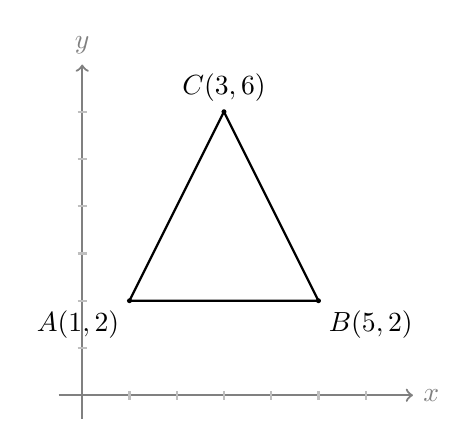
\begin{tikzpicture}[scale=0.6, thick]
  \draw[gray, ->] (-0.5, 0) -- (7, 0) node[right] {$x$};
  \draw[gray, ->] (0, -0.5) -- (0, 7) node[above] {$y$};
  \foreach \x in {1,2,3,4,5,6} \draw[gray!50] (\x, -0.1) -- (\x, 0.1);
  \foreach \y in {1,2,3,4,5,6} \draw[gray!50] (-0.1, \y) -- (0.1, \y);

  \coordinate (A) at (1, 2);
  \coordinate (B) at (5, 2);
  \coordinate (C) at (3, 6);

  \draw (A) -- (B) -- (C) -- cycle;
  \fill (A) circle (1.5pt); \node[below left] at (A) {$A(1,2)$};
  \fill (B) circle (1.5pt); \node[below right] at (B) {$B(5,2)$};
  \fill (C) circle (1.5pt); \node[above] at (C) {$C(3,6)$};
\end{tikzpicture}
\end{document}
